\section{Evaluation}
\subsection{Security}
\begin{frame}{Security of the PIN Component (1 of 3)}
\begin{itemize}
	\item<1-> Let's consider an attacker Oscar, who is trying to gain unauthorized access to a door by exploiting weaknesses inherent to a certain authentication factor used in the system.
    \item<2-> The main security concern with PIN is its vulnerability to brute force attacks.
    \item<3-> If an attacker Oscar gets hold of an authorized RFID tag, he can gain access to a door if he guesses the corresponding PIN.
    \item<4-> However, a lockout functionality has been implemented for RFID authentication, so Oscar has to wait a long time between guesses.
\end{itemize}
\end{frame}

\begin{frame}{Security of the PIN Component (2 of 3)}
\begin{itemize}
	\item<1-> The following formula is the average time it takes to guess a PIN using brute force in the system:
	$$T = (g \cdot t) + (L \cdot \frac gn) $$
	\item<2-> Where:
	\begin{itemize}
		\item<3-> $g$ is the average number of guesses needed
		\item<4-> $t$ is the average time it takes to try out a single PIN
		\item<5-> $L$ is the waiting time after a single lock-out
		\item<6-> and $n$ is the number of wrong attempts it takes before being locked-out.
	\end{itemize}
\end{itemize}
\end{frame}

\begin{frame}{Security of the PIN Component (3 of 3)}
\begin{itemize}
	\item<1-> On average, Oscar only needs to enter half of all possible PINs before guessing the correct one.
	\item<2-> There is no maximum PIN length imposed, which means the number of possible PINs is theoretically infinite, but assuming the following:
	\begin{itemize}
		\item<3-> All users use 6-digit PINs
		\item<4-> It takes 5 seconds to try out a single PIN.
		\item<5-> Lockout time is 30 minutes (default) 
		\item<6-> Attempt limit is 5 (default) 
	\end{itemize}
	\item<7-> Hence, $ g = \frac12 \cdot 10^6 = 500,000 \:\mathrm{guesses}, t = 5 \:\mathrm{s}, L = 1800 \:\mathrm{s}, n = \mathrm{5}$
	\item<8-> Plugging in those values, it would take, on average, $50694$ hours, or about $5.78$ years to crack. This makes brute force an impractical attack to use.
\end{itemize}
\end{frame}

\begin{frame}{Security of the RFID Component (1 of 2)}
\begin{itemize}
    \item<1-> The primary concern with RFID security is the issue of stolen or replicated tags.
    \item<2-> While we cannot prevent tags from being stolen, this is not a problem because our system allows admins to edit or deactivate keypairs.
    \item<3-> Hence, the user simply needs to go to the admin to get his keypair changed or deactivated.
\end{itemize}
\end{frame}

\begin{frame}{Security of the RFID Component (2 of 2)}
\begin{itemize}
    \item<1-> Replication of an RFID tag can be performed by scanning its UID, and reprogramming another tag to have the same UID.
    \item<2-> Attackers do not need to have access to the actual tag, as they can find out the UID simply by placing keyloggers near the RFID reader and waiting for it to be scanned.
    \item<3-> The MiFare cards we used cannot have their UIDs reprogrammed \footfullcite{MiFareAdafruit}, but some MiFare cards are made specially for cloning purposes (called ``magic'' MiFare cards).
    \item<4-> MiFare in general is not known to be secure, as some attacks have been developed for it. De Koning Gans et al recommend that a more advanced RFID card technology with an open design architecture be used over MiFare \footfullcite{de2008practical}.
\end{itemize}
\end{frame}

\begin{frame}{Security of the Fingerprint Component (1 of 2)}
\begin{itemize}
    \item<1-> The problem with fingerprint security is the possibility of generating false positives and false negatives. 
    \item<2-> While a false negative (denying a user that is supposed to be authorized) might cause some minor inconvenience on the part of the user, a false positive (allowing a user that is not supposed to be authorized) is potentially devastating.
    \item<3-> However, an attacker cannot rely solely on chance in order to generate a false positive, since that probability is infinitesimally small (less than 0.00001\% in our case).
\end{itemize}
\end{frame}

\begin{frame}{Security of the Fingerprint Component (2 of 2)}
\begin{itemize}
    \item<1-> What the attacker can do is to make a clone of the registered fingerprint. This can be done by pressing the finger against various materials such as silicone or gelatin, in order to make a mold.
    \item<2->  We have not personally tested our fingerprint scanner against such clones, but in the study done by Matsumoto et al on 11 fingerprint scanners, they found that 67\% of them accepted the gummy fingers \footfullcite{matsumoto2002impact}.
    \item<3-> Hence, it is not unreasonable to assume that our scanner will also be deceived by artificial fingers.
    \item<4-> However, this attack relies on the attacker obtaining an accurate mold of the finger, which usually requires the cooperation and consent of the authorized user.
\end{itemize}
\end{frame}

\begin{frame}{Security Against Passive Attacks (1 of 2)}
\begin{itemize}
    \item<1-> Let us assume that an eavesdropper Eve can read all messages being passed between SpoonPi and ForkPi, and ForkPi and the admin’s computer.
    \item<2-> While Eve can listen in on the exchanges, she cannot modify them.
    \item<3-> Hence, our system is secure against such attacks for both communication lines.
    \item<4-> \textbf{Communication between SpoonPi and ForkPi}: When a PIN is entered or an RFID UID is scanned, SpoonPi never queries for matches in plaintext. These two fields are hashed first using SHA-1, so Eve cannot retrieve their original values.
\end{itemize}
\end{frame}

\begin{frame}{Security Against Passive Attacks (2 of 2)}
\begin{itemize}
    \item<1-> \textbf{Communication between ForkPi and the admin’s computer}:
    \begin{itemize}
    	\item<2-> In the web application, it becomes more difficult to safely transmit the PIN and RFID UID without exposing them to Eve, since admins need to be able to view them in plaintext.
    	\item<3-> When an admin logs in, the authentication credentials are not included in the web page. However, when the admin edits a user’s keypair, his/her credentials will be sent to ForkPi in plaintext.
    	\item<4-> The same goes for when the admin adds a new keypair; the new keypair’s credentials might be exposed to Eve. The impact is lessened in a system with multiple doors, since it would become more difficult for Eve to determine which door(s) a keypair is linked to.
    \end{itemize}
\end{itemize}
\end{frame}

\begin{frame}{Security Against Active Attacks (1 of 3)}
\begin{itemize}
    \item<1-> Let us assume that a malicious attacker, Mallory, is actively trying to break into the security of the system, either by targeting a single computer, or by pretending to be a certain computer to another computer.
\end{itemize}
\end{frame}

\begin{frame}{Security Against Active Attacks (2 of 3)}
\begin{itemize}
    \item<1-> \textbf{Attack on the Database}:
    \begin{itemize}
    	\item<2-> If Mallory was able to guess the username and password of the PostgreSQL database, she would gain access to it.
    	\item<3-> However, she will not be able to retrieve the PIN and RFID UID in plaintext, since they are encrypted in 128-bit AES.
    	\item<4-> Gaining access to the database can still potentially damage the system because Mallory can delete all the tables and rows. This is a severe attack on the system, so it is highly recommended to have a strong username and password for PostgreSQL.
    \end{itemize}
\end{itemize}
\end{frame}

\begin{frame}{Security Against Active Attacks (3 of 3)}
\begin{itemize}
    \item<1-> \textbf{Man In The Middle Attack}:
    \begin{itemize}
    	\item<2-> All computers in the local network refer to ForkPi using \texttt{forkpi.local}
    	\item<3-> Theoretically, Mallory can create a naming collision with ForkPi by setting her own computer’s hostname to forkpi, and then running a service under the name \texttt{forkpi.local}.
    	\item<4-> However, the service discovery software that we use, Avahi, resolves name collisions by appending a number to the hostname (e.g. \texttt{forkpi-2.local}), in accordance with the Zeroconf protocol \footfullcite{rfc6762}.
    	\item<5-> These numbers are assigned according to the order of start-up. Hence, provided that the ForkPi unit is started before Mallory's computer, \texttt{forkpi.local} will refer to the real ForkPi unit. Therefore, it will be hard for Mallory to pass off her own computer as the ForkPi unit.
    \end{itemize}
\end{itemize}
\end{frame}

\subsection{Usability}
\begin{frame}{Usability (1 of 4)}
\begin{itemize}
    \item<1-> The following figure shows the list of questions and the amount of respondents for each possible response.
    \item<2-> 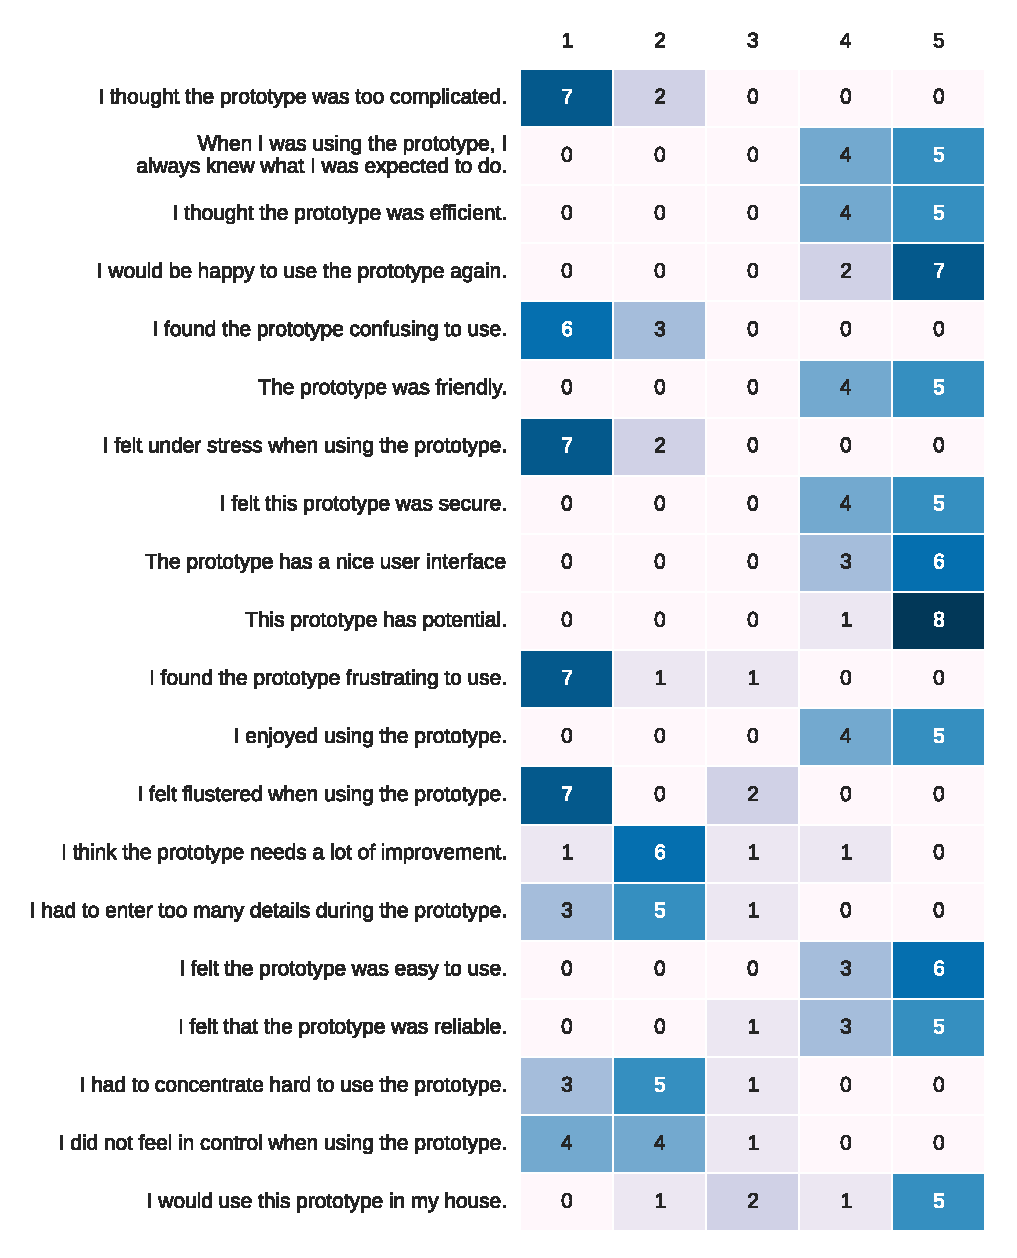
\includegraphics[scale=0.25]{uat-results.eps}
\end{itemize}
\end{frame}
\begin{frame}{Usability (2 of 4)}
\begin{itemize}
    \item<1-> Some of the questions were phrased negatively in order to ensure that the respondents are reading the questions carefully.
    \item<2-> There was a total of nine respondents from different walks of life:
    \begin{itemize}
        \item<3-> Four of the respondents were female, while five were male.
        \item<4-> Four of the respondents were within the 18 to 25 age range, the other four were within the 26 to 40 age range, and the remaining respondent was aged 68.
    \end{itemize}
\end{itemize}
\end{frame}

\begin{frame}{Usability 3 of 4)}
\begin{itemize}
    \item<1-> The following figure shows the list of respondents and their answers, grouped by their answer to the question, ``Have you ever operated/used a door access control system before?''
    \item<2-> 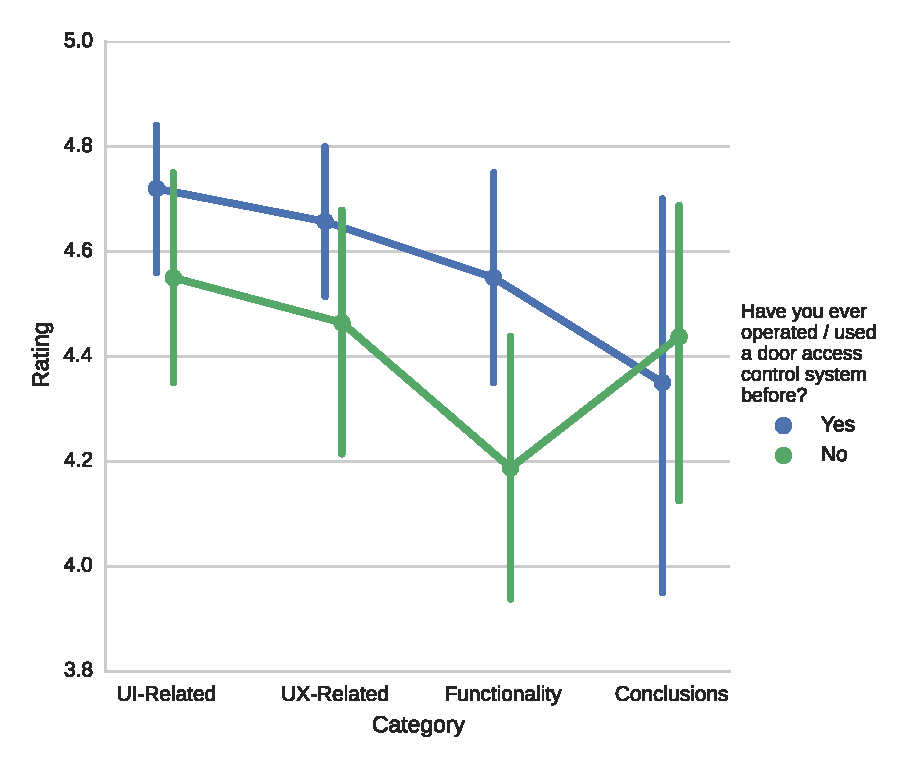
\includegraphics[scale=0.7]{tech-non-tech.eps}
\end{itemize}
\end{frame}

\begin{frame}{Usability 4 of 4)}
\begin{itemize}
    \item<1-> Five of the respondents had no experience at all with keyless door access control systems.
    \item<2-> The respondents who had no experience reviewed the system less favorably, as opposed to the respondents who had experience.
    \item<3-> An exception, however, occurs with questions pertaining to drawing conclusions from the system (e.g. ``The prototype has potential.''), where the respondents with no experience ranked the system more favorably.
    \item<4-> Overall, the respondents rated the system positively, commenting that the system shows promise and has a lot of potential, especially compared to products that are currently in the market.
\end{itemize}
\end{frame}

\subsection{Cost-Effectiveness}
\begin{frame}{Cost-Effectiveness (1 of 3)}
\begin{itemize}

    \item<1-> In this section, we list all the hardware components we used for the system, along with their respective prices.
    \item<2-> We then compare the prices of each component against the prices of similar components that can be purchased from the online store Amazon \footfullcite{Amazon}.
    \item<3-> We also compare the total price of our system against similar commercial products that are for sale on Amazon.
    
\end{itemize}
\end{frame}

\begin{frame}{Cost-Effectiveness (2 of 3)}
\begin{itemize}

    \item<1-> In determining the price ranges, we took a look at the price filters on Amazon, and for each price range, we multiplied the number of items by the maximum amount in that range. (e.g.: For the \$200 and above price, we set the price to \$250.)
    \item<2-> In determining the lower end of the range, we set the count of the most expensive group to 0, and took the mean price. For the higher end, we set the count of the least expensive group to 0, and took the mean price.
    
\end{itemize}
\end{frame}

\begin{frame}{Cost-Effectiveness}
\begin{table}[h]
	\centering
	\begin{threeparttable}
	\begin{tabular}{lll|l|l|}
	\cline{4-5}
	 &  &  & \multicolumn{2}{c|}{Cost} \\ \hline
	\multicolumn{1}{|l|}{} & \scriptsize{Component} & & \scriptsize{Project} & \scriptsize{Commercial} \\ \hline
	\multicolumn{1}{|l|}{Base} & \scriptsize{Raspberry Pi Model B} &  & \scriptsize{\$35} & \scriptsize{\$35} \\
	\multicolumn{1}{|l|}{} & \scriptsize{OLED Display} &  & \scriptsize{\$17.50} & \scriptsize{\$10 - \$20} \\
	\multicolumn{1}{|l|}{} & \scriptsize{Raspberry Pi Cobbler Breakout} &  & \scriptsize{\$6.50} & \scriptsize{\$6 - \$11} \\ \hline
	\multicolumn{1}{|l|}{PIN} & \scriptsize{Keypad} &  & \scriptsize{\$3.95} & \scriptsize{\$2.5 - \$7} \\ \hline
	\multicolumn{1}{|l|}{RFID} & \scriptsize{Reader} &  & \scriptsize{\$39.95} & \scriptsize{\$30 - \$80} \\
	\multicolumn{1}{|l|}{} & \scriptsize{MiFare Classic 13.56MHz Card x1} &  & \scriptsize{\$2.50} & \scriptsize{\$0.5 - \$1.5} \\
	\multicolumn{1}{|l|}{} & \multicolumn{2}{r|}{\scriptsize{Total (Base+RFID+PIN)}} & \scriptsize{\$102.9} & \scriptsize{\$80 - \$140} \\ \hline
	\multicolumn{1}{|l|}{Fingerprint} & \scriptsize{Scanner} &  & \scriptsize{\$49.95} & \scriptsize{\$40 - \$90} \\
	\multicolumn{1}{|l|}{} & \multicolumn{2}{r|}{\scriptsize{Total (Base+Fingerprint+PIN)}} & \scriptsize{\$110.4} & \scriptsize{\$100 - \$170} \\ \hline
	\multicolumn{1}{|l|}{} & \multicolumn{2}{r|}{\scriptsize{Total (All Components)}} & \scriptsize{\$152.85} & \scriptsize{\$140 - \$200} \\ \hline
	\end{tabular}
	\end{threeparttable}
	\end{table}

\end{frame}